\documentclass[12pt,a4paper]{article}
\usepackage[utf8]{inputenc}
\usepackage{amssymb, amsthm, multicol}
\usepackage[russian]{babel}
\usepackage{tikz}
\thispagestyle{empty}

\oddsidemargin=-15.4mm
\textwidth=190mm
\headheight=-32.4mm
\textheight=277mm
\tolerance=100
\parindent=0pt
\parskip=8pt


\begin{document}
\begin{center}
\textbf{ТЕОРИЯ ГРАФОВ}
\end{center}

	Первым упоминанием графов считается письмо Леонарда Эйлера, написанное в 1736 году, в котором он решил известную <<Задачу о семи кёнигсбергских мостах>>. За 280 лет теория графов эволюционировала: её содержание приобрело необыкновенную стройность, познания в этой области сильно углубились, а главное~---~специалисты из многих областей, далёких от математики, поняли, что граф~---~один из самых мощнейших инструментов, который ускоряет процесс исследований.
	
	Сейчас применение теории графов можно найти и в теории шифрования, и в теории алгоритмов, и в экономике, и в социологии, и в многих других областях. Ежегодно выходит громадное число пособий, раскрывающих ту или иную сторону теории графов; в большинстве своём эти пособия имеют свою специализированную аудиторию и не рассчитаны на широкую публику.
	
	В свою очередь, цель этого курса: познакомить начинающего с базовыми знаниями этой теории, открыть любителям математики красивые стороны теории графов и познакомить знатоков этой теории с интересными и сложными теоремами, позволяющими взломать большое число олимпиадных задач. Сначала мы познакомимся с простейшими видами графов и решим задачи на эту тематику, а потом поговорим об их применении в реальных ситуациях.
	
	В программе: лемма о рукопожатиях, деревья, связные графы, изоморфизмы, планарные графы, формула Эйлеры, эйлеровы и гамильтоновы циклы, ориентированные графы, двудольные графы, лемма Холла. Вводная лекция будет посвящена истории становления теории графов и заключительная лекция о практическом применении графов.
	
\begin{center}
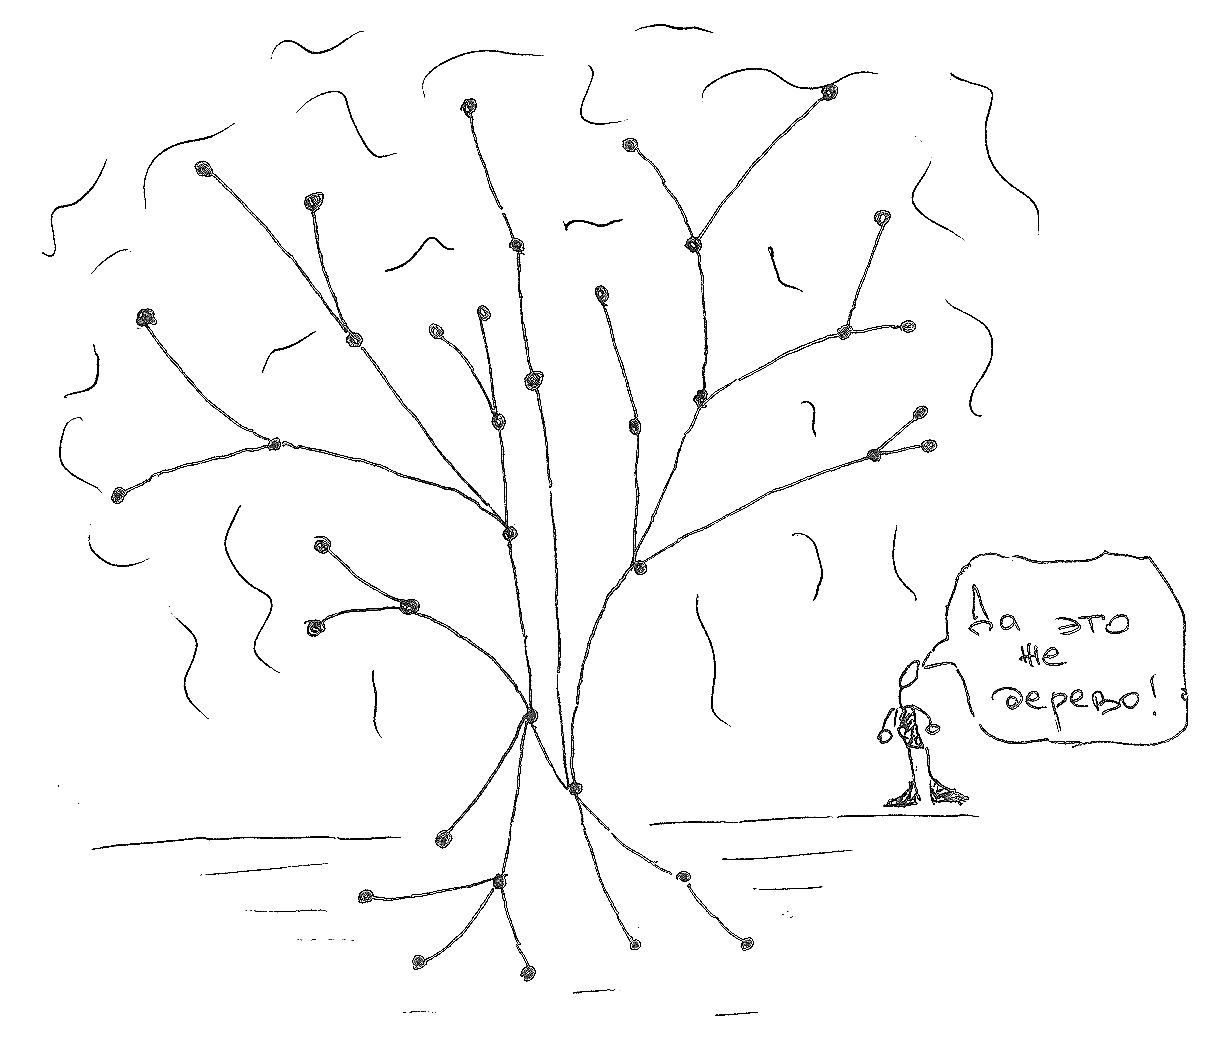
\includegraphics[width=20cm, height=12cm,keepaspectratio]{tree}
\end{center}
\end{document}